\section{Benutzeroberfläche}
Anbei sind exemplarisch Entwürfe einer möglichen Umsetzung der Benutzeroberfläche eingefügt. 

Die Benutzeroberfläche besteht aus verschiedenen Bereichen. 
Die Oberfläche hat einen Header (orange). 
Jede aufrufbare Seite der App hat ein Titel, der auf dem Header angezeigt wird.
Außerdem hat jede Seite verschiedene Elemente:
\begin{itemize}[nosep]
	\item Hintergrund (weiß)
	\item Textuelle Beschreibungen (schwarz)
	\item Eingabefelder (grau)
	\item Buttons (blau)
	\item Bilder (grün)
\end{itemize}

\subsection{Menü, Header und Suche}

\begin{figure}[H]
	\begin{minipage}[c]{.5\textwidth} 
		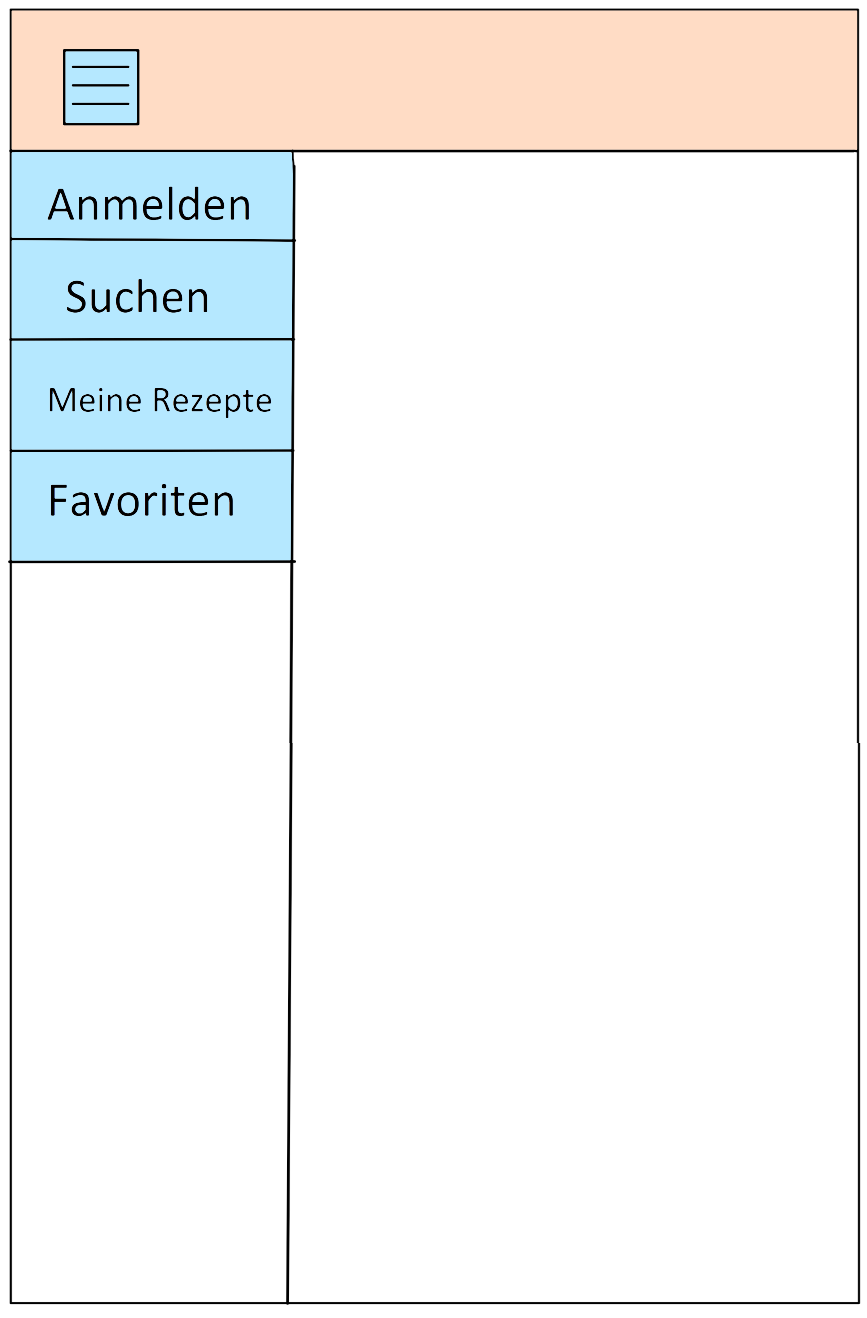
\includegraphics[width=\textwidth]{gui/seitenmenue.png}			
		\caption{Seitlich angezeigtes Menü der App}
		\label{menü}
	\end{minipage} \hspace{.7cm}
	\begin{minipage}[c]{.5\textwidth} 
			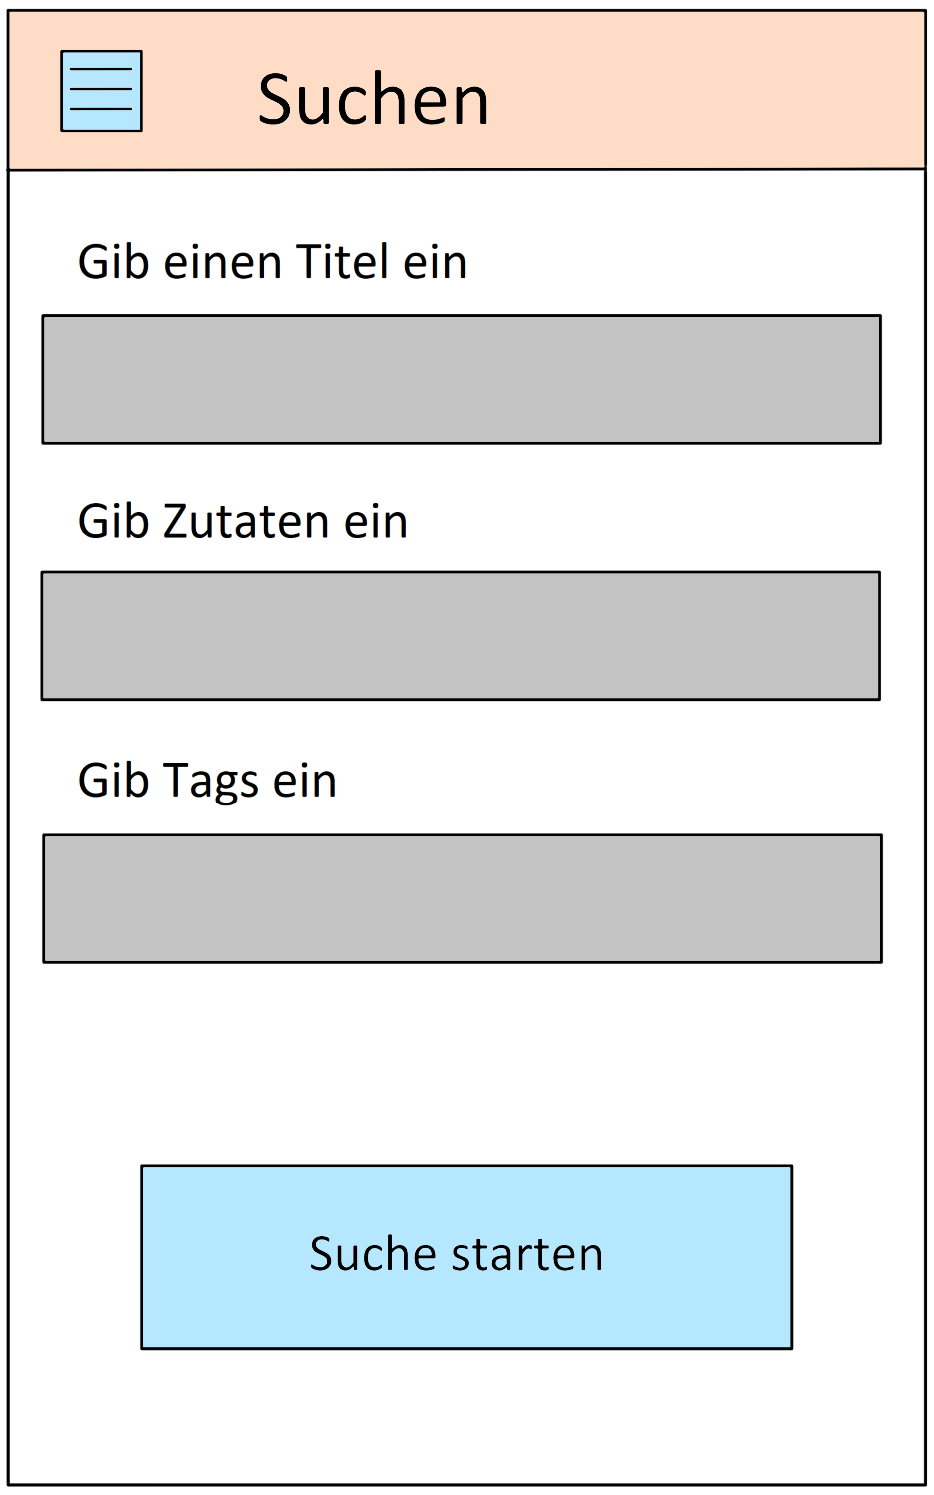
\includegraphics[width=\textwidth]{gui/suchen.png}				
		\caption{Suchfunktion mit Eingabefeldern und Buttons}
		\label{suche}
	\end{minipage}
\end{figure}


Das Menü in \ref{menü} zeigt die aufrufbaren Seiten der App. Es kann durch Klicken auf den Menübutton oben links auf dem Header ein- und ausgeblendet werden. Die Reiter im Menü sind Buttons, welche auf die jeweilig genannte Seite der App führen. Das Menü ist von jeder Seite der App aus erreichbar. Der Header ist ebenfalls immer über jeder Seite sichtbar. 

Skizze \ref{suche} zeigt die Suchfunktion. Nutzer können \gls{Suchfilter} in die Textfelder eingeben und die Suche dann starten. Die Suchseite ist auch die Startseite der App. Also die, die angezeigt wird, wenn ein Nutzer die App startet.


\subsection{Anmelden}

\begin{figure}[H]
	\begin{minipage}[c]{.5\textwidth} 
		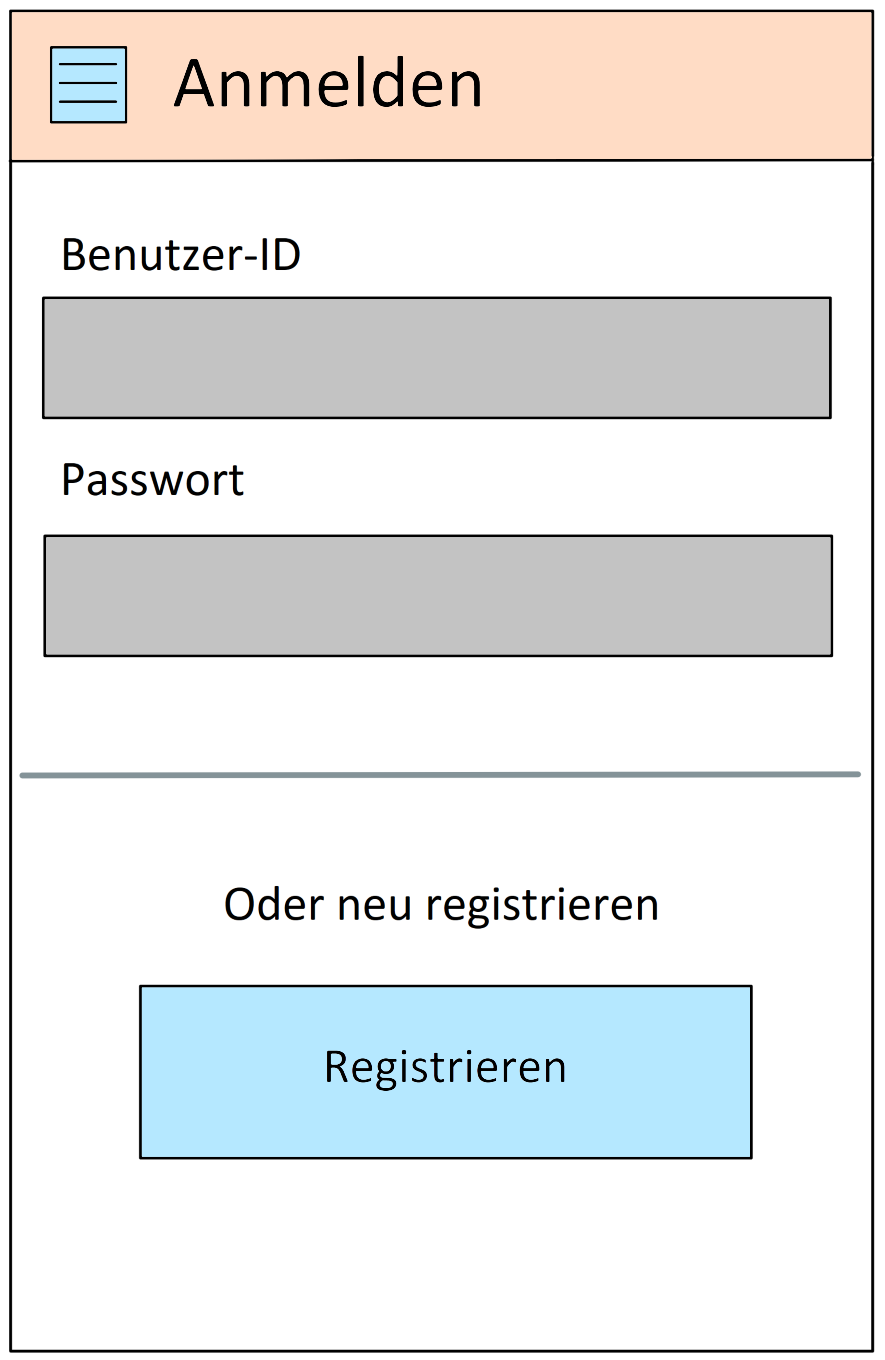
\includegraphics[width=\textwidth]{gui/anmelden.png}			
		\caption{Login-Seite}
		\label{anmelden}
	\end{minipage} \hspace{.7cm}
	\begin{minipage}[c]{.5\textwidth} 
			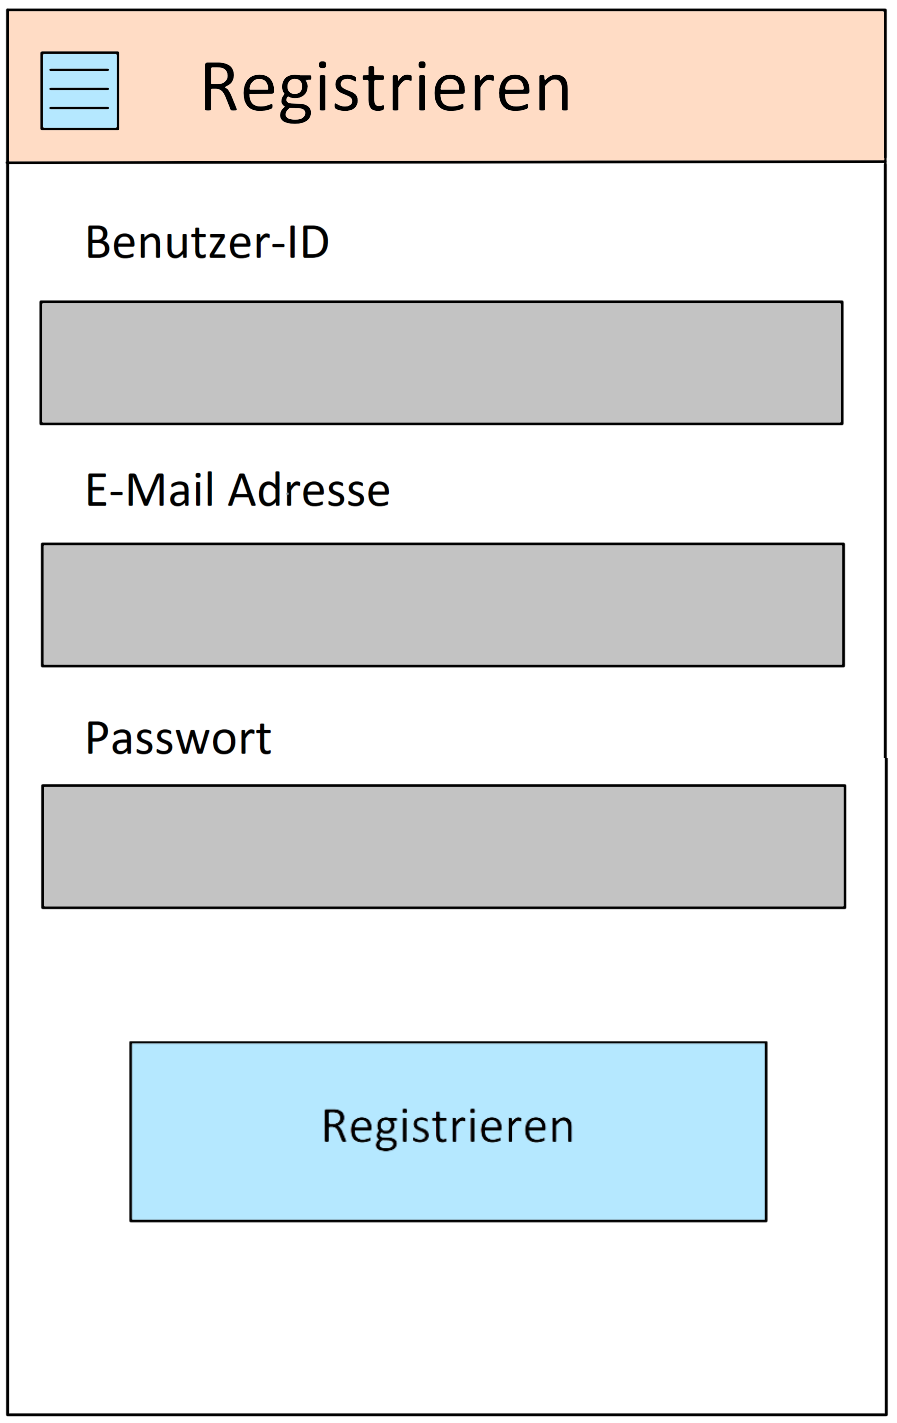
\includegraphics[width=\textwidth]{gui/registrieren.png}				
		\caption{Registrierung eines neuen Nutzers}
		\label{registrieren}
	\end{minipage}
\end{figure}

Die Login-Seite, die in \ref{anmelden} zu sehen ist, zeigt zwei Textfelder, in die der Nutzer die erforderlichen Anmeldeinformationen eintragen kann. Ist ein Nutzer noch nicht registriert, kommt er über den "`Registrieren"'-Button zur entsprechenden Seite.

Von der Login-Seite aus, kann ein Nutzer die Registrierungsseite erreichen, wie sie in \ref{registrieren} zu sehen ist. Hier kann er die nötigen Daten zur Registrierung angeben. Ist er fertig, drückt er auf den Button und wird in die Datenbank aufgenommen.



\subsection{Meine Rezepte}

\begin{figure}[H]
	\begin{minipage}[c]{.5\textwidth} 
		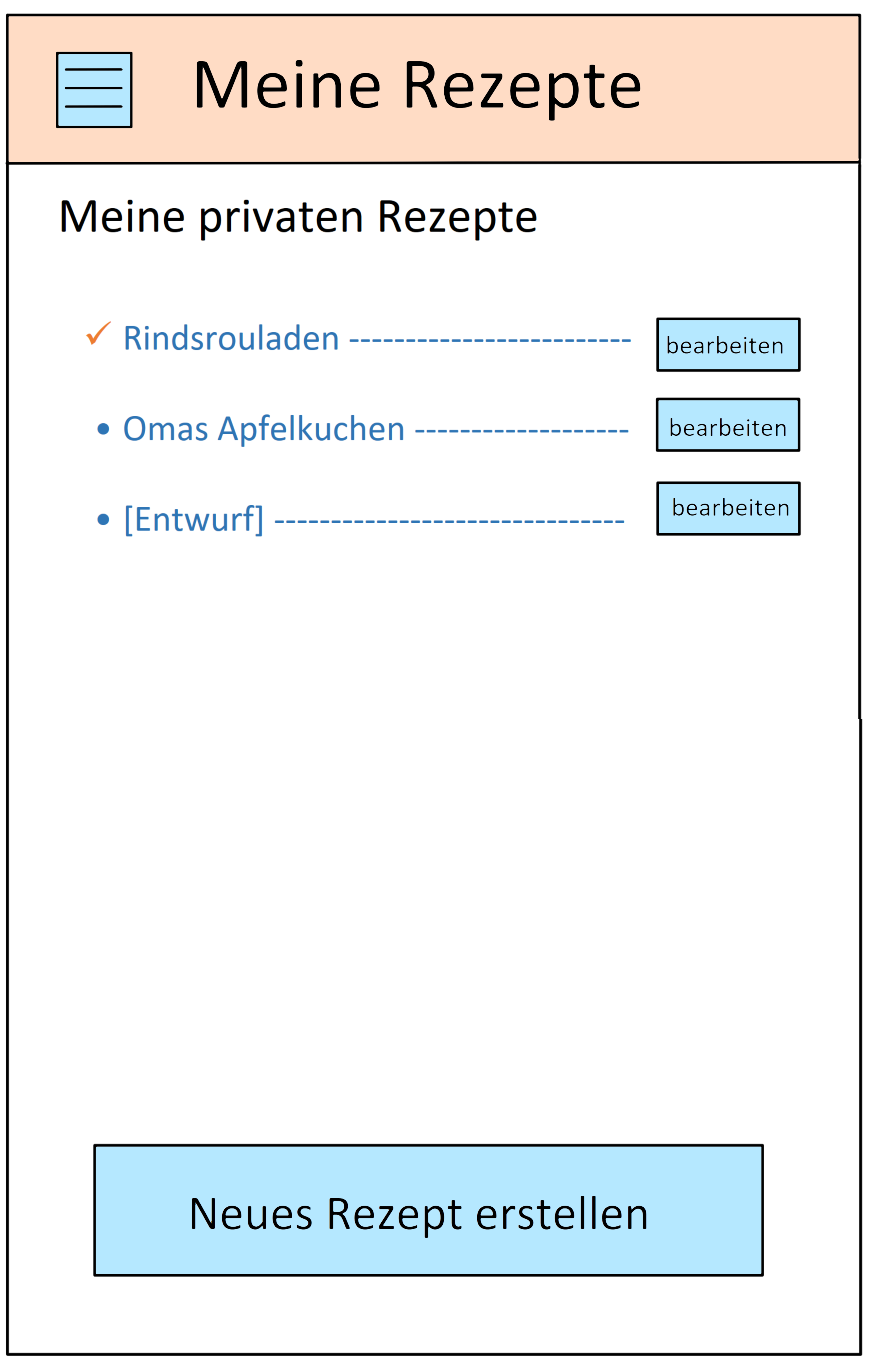
\includegraphics[width=\textwidth]{gui/meine_rezepte.png}	
		\caption{Abschnitt mit privaten und veröffentlichten Rezepten}
		\label{rezeptliste}
	\end{minipage} \hspace{.7cm}
	\begin{minipage}[c]{.5\textwidth} 
			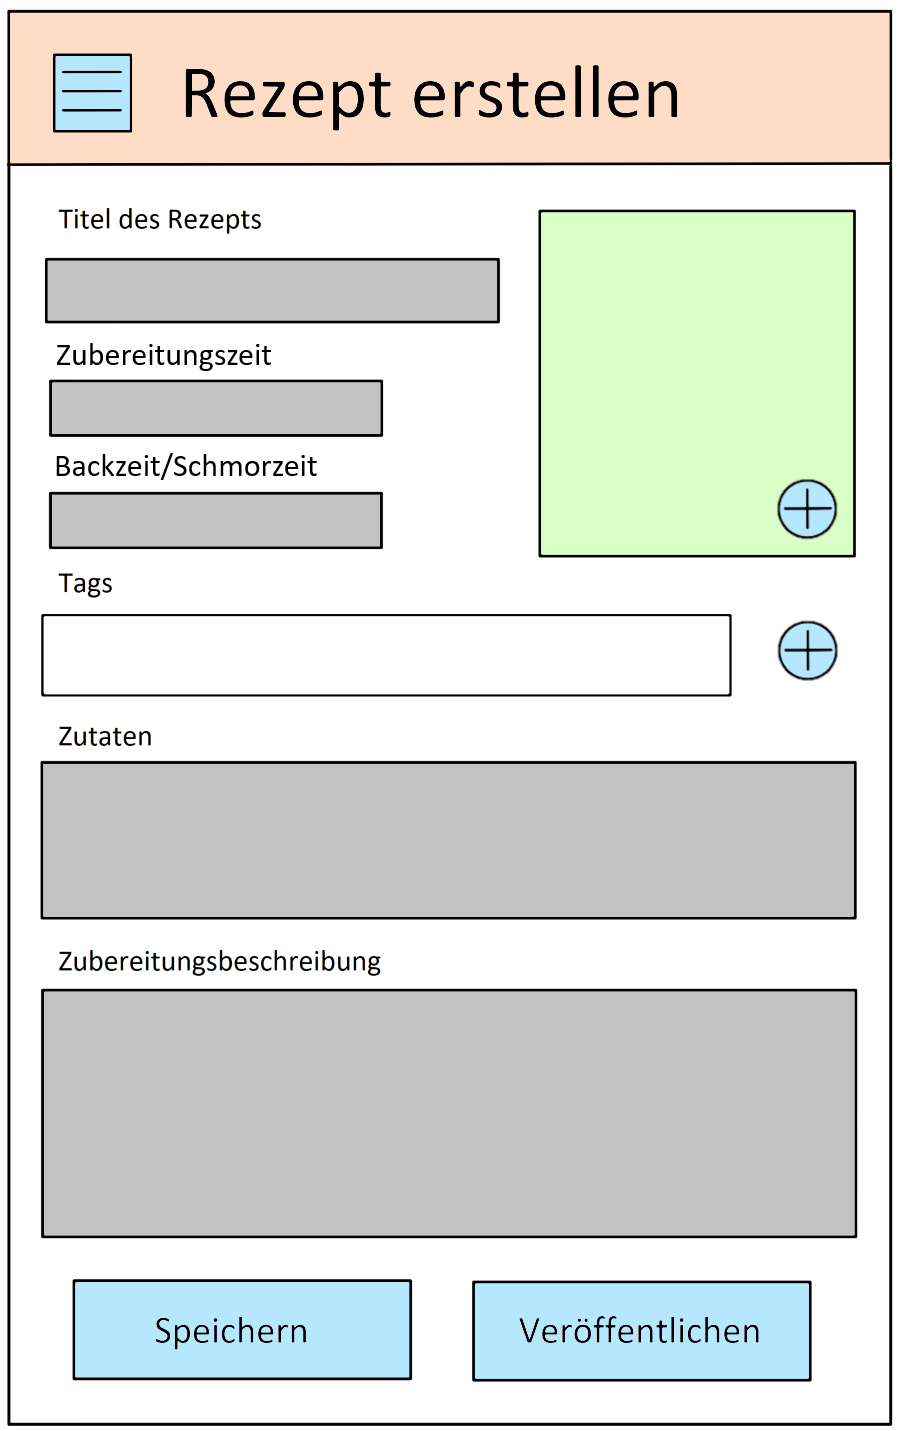
\includegraphics[width=\textwidth]{gui/rezept_erstellen.png}				
		\caption{Neues Rezept erstellen}
		\label{erstellen}
	\end{minipage}
\end{figure}


Abbildung \ref{rezeptliste} zeigt den Abschnitt "`Meine privaten Rezepte"'. Hier werden die Titel der Rezepte aus der \gls{Rezeptliste} eines Nutzers angezeigt. Rezepte, die noch keinen Titel haben, werden mit einem Platzhalter (hier: [Entwurf]) markiert. 
\Glspl{oRezept} haben dabei ein Häkchen, \glspl{pRezept} einen runden Punkt als führendes Icon. 
Über den "`bearbeiten"'-Button kann ein Rezept bearbeitet werden. 
Soll ein neues Rezept erstellt werden, kann der Nutzer das über den Button tun.

In \ref{erstellen} erstellt der Nutzer gerade ein neues Rezept. Er kann in die Textfelder entsprechende Informationen eintragen und über den runden Button im Bildfenster ein Bild hinzufügen. \glspl{Tag} kann er über den unteren runden Button neben dem "`\glspl{Tag}"'-Feld hinzufügen. Möchte er sein Rezept veröffentlichen, so klickt er auf "`Veröffentlichen"'. Hat der Nutzer das Rezept bereits veröffentlicht, zeigt dieser Button stattdessen "`Aktualisieren"' an. Der "`Speichern"'-Button gibt ihm die Möglichkeit, das Rezept manuell zu speichern. 

